% ALGUNOS PAQUETES REQUERIDOS (EN UBUNTU): %
% ========================================
% %
% texlive-latex-base %
% texlive-latex-recommended %
% texlive-fonts-recommended %
% texlive-latex-extra %
% texlive-lang-spanish (en ubuntu 13.10) %
% ******************************************************** %

\documentclass[a4paper]{article}
\usepackage[spanish]{babel}
\usepackage[utf8]{inputenc}
\usepackage{fancyhdr}
\usepackage[pdftex]{graphicx}
\usepackage{sidecap}
\usepackage{caption}
\usepackage{subcaption}
\usepackage{booktabs}
\usepackage{makeidx}
\usepackage{float}
\usepackage{amsmath, amsthm, amssymb}
\usepackage{amsfonts}
\usepackage{sectsty}
\usepackage{wrapfig}
\usepackage{listings}
\usepackage{enumitem}
\usepackage{hyperref}
\usepackage{listings}
\usepackage{listingsutf8}

% Para ver los marcos
% \usepackage{showframe}

\newcommand{\ord}{\ensuremath{\operatorname{O}}}
\newcommand{\nat}{\ensuremath{\mathbb{N}}}
\renewcommand{\thesubsubsection}{\thesubsection.\alph{subsubsection}}

% Lemas, definiciones, etc.
\theoremstyle{remark}
\newtheorem*{obs}{Observación}
\newtheorem*{nota}{Notación}
\theoremstyle{plain}
\newtheorem{teo}{Teorema}
\newtheorem{lema}{Lema}
\newtheorem{prop}{Propiedad}
\usepackage{color} % para snipets de codigo coloreados
\usepackage{fancybox}  % para el sbox de los snipets de codigo

\definecolor{litegrey}{gray}{0.94}

% \newenvironment{sidebar}{%
% 	\begin{Sbox}\begin{minipage}{.85\textwidth}}%
% 	{\end{minipage}\end{Sbox}%
% 		\begin{center}\setlength{\fboxsep}{6pt}%
% 		\shadowbox{\TheSbox}\end{center}}
% \newenvironment{warning}{%
% 	\begin{Sbox}\begin{minipage}{.85\textwidth}\sffamily\lite\small\RaggedRight}%
% 	{\end{minipage}\end{Sbox}%
% 		\begin{center}\setlength{\fboxsep}{6pt}%
% 		\colorbox{litegrey}{\TheSbox}\end{center}}

\newenvironment{codesnippet}{%
	\begin{Sbox}\begin{minipage}{\textwidth}\sffamily\small}%
	{\end{minipage}\end{Sbox}%
		\begin{center}%
		\vspace{-0.4cm}\colorbox{litegrey}{\TheSbox}\end{center}\vspace{0.3cm}}



\usepackage{fancyhdr}
% \pagestyle{fancy}
%\renewcommand{\chaptermark}[1]{\markboth{#1}{}}
\renewcommand{\sectionmark}[1]{\markright{\thesection\ - #1}}
\fancyhf{}
% \fancyhead[LO]{Sección \rightmark} % \thesection\

% \fancyfoot[RO]{\thepage}
\renewcommand{\headrulewidth}{0.5pt}
\renewcommand{\footrulewidth}{0.5pt}
%\setlength{\hoffset}{-0.8in}
\setlength{\textwidth}{16cm}
\setlength{\hoffset}{-1.1cm}
\setlength{\headsep}{0.5cm}
\setlength{\textheight}{25cm}
\setlength{\voffset}{-0.7in}
\setlength{\headwidth}{\textwidth}
\setlength{\headheight}{13.1pt}
\renewcommand{\baselinestretch}{1.1} % line spacing


\begin{document}

\title{Algoritmos y Estructuras de Datos III}
\author{Manuel Mena}
\maketitle

\tableofcontents

\newpage
\section{Teoremas, lemas y propiedades}

\subsection{Propiedades básicas}

\begin{lema}
\label{aristasGrados}
    Sea $G$ un grafo con $m$ aristas y $n$ nodos, se verifica que $m = \frac{\sum_{i = 1}^{n}d(v_i)}{2}$.
\end{lema}

\begin{prop}
\label{compConexo}
    $G$ no conexo $\Longrightarrow \overline{G}$ es conexo.
\end{prop}

\begin{prop}
\label{n5CicloConexo}
    Si $n \geq 5 \Longrightarrow \overline{C_n}$ es conexo.
\end{prop}

\subsection{Árboles}

\begin{lema}
\label{eCircSimple}
    $G = (V, X)$ grafo conexo y $e \in X$. $G - e$ es conexo
    $\Longleftrightarrow e \in$ circuito simple de $G$.
\end{lema}

\begin{proof}
    ~

    $\Longrightarrow$ )

    $G$ es conexo, $e \in X$, $e:(v, w)$

    $G - e$ es conexo, entonces existe un camino simple $P$ entre $v$ y $w$ en
    $G - e$.

    Entonces $P + e$ es un circuito simple en $G$

    ~

    $\Longleftarrow$ )

    $e \in$ circuito simple de $G$, $C$

    Sean $z_1, z_2 \in V$. Seguro existe en $G$ un camino entre $z_1$ y $z_2$.
    Si ese camino no usa $e$, ese camino también pertenece a $G - e$. Si usa
    $e$, armamos un nuevo camino donde reemplazamos $e$ por $C - e$, donde el
    camino resultante $\in G - e \Longrightarrow G - e$ conexo.
\end{proof}

\begin{lema}
\label{concatCircSimple}
    La concatenación de dos caminos distintos entre un par de vértices contiene un circuito simple.
\end{lema}

\begin{teo}
    Dado un grafo $G = (V, X)$ son equivalentes:

    \begin{enumerate}
        \item $G$ es un árbol.
        \item $G$ es un grafo sin circuitos simples, pero si se agrega
        cualquier arista $e$ a $G$resulta un grafo con exactamente un circuito
        simple, y ese circuito contiene a $e$.
        \item Existe exactamente un camino simple entre todo par de nodos.
        \item $G$ es conexo, pero si se quita cualquier arista a $G$, queda un
        grafo no conexo.
    \end{enumerate}
\end{teo}

\begin{proof}
~

1) $\Longrightarrow$ 2)

$G$ árbol por definición $\Longrightarrow G$ conexo y sin ciclos simples sea $e \notin G$, $G + e$ es conexo.

$(G + e) - e = G$ es conexo, entonces por Lema \ref{eCircSimple}, $e$ pertenece a un circuito simple de $G + e$.

Falta ver que sólo hay un circuito en $G + e$. Si hay en $G + e$ algún circuito al cual $\notin e$, ese circuito también estaría en $G$. Pero no puede ser porque $G$ es árbol.

Si hay 2 o más circuitos en $G + e$, como $e$ tiene que pertenecer a todos, $C_1 - e$ es camino entre ``las puntas'' de $e$ y $C_2 - e$ es otro. Por Lema 2 $(C_1 - e) + (C_2 + e)$ contiene un circuito simple que pertenecería a $G$. Pero no puede ser porque $G$ es árbol. 

~

2) $\Longrightarrow$ 3)

Sea $G$ que cumple 2). Suponemos que para $v, w$ no existe camino. $G + (v, w)$ tiene ciclo al cual $\in (v, w) + C$. Pero entonces $C - (v, w)$ es camino entre $v$ y $w$ en $G$. Absurdo. Entre todo par de vértices por lo menos existe un camino.

Supongo que existen dos caminos distintos entre $v$ y $w$. Por Lema \ref{concatCircSimple} la concatenación de esos caminos contiene un circuito. Absurdo porque $G$ no tiene circuitos.

~

3) $\Longrightarrow$ 4)

$G$ cumple 3). $G$ es conexo.

Sean $u, v$ dos vértices cualquiera y $e$ una arista del único camino simple entre $u$ y $v$ en $G$. Entonces en $G - e$ no existe un camino entre $u$ y $v$. Por lo tanto $G - e$ no es conexo.

~

4) $\Longrightarrow$ 1)

$G$ cumple 4), entonces es conexo.

Si hubiese un circuito en $G$, por Lema \ref{eCircSimple} al sacar una arista de ese circuito el grafo seguiría siendo conexo. Absurdo porque $G$ cumple 4) $\Longrightarrow G$ es árbol.
\end{proof}
\begin{lema}[Hojas]
\label{hojas}
    Todo árbol no trivial tiene al menos dos hojas
\end{lema}

\begin{proof}
    Sea $P$ un camino ``no extensible en los extremos'' (no incluido en un camino más grande), llamamos $u$ y $v$ a los extremos del camino.

    No puede estar fuera del camino porque $P$ es maximal, no puede estar dentro ya que por Lema \ref{concatCircSimple}, se formaría un ciclo.
\end{proof}

\begin{lema}
    Sea $G = (V, X)$ un árbol, entonces $m = n - 1$
\end{lema}

\begin{proof}
    ~

    Inducción en $n$:

    Caso base: $n = 1$ $m = 0 = 1 - 1 = n - 1$

    Paso inductivo ($n \geq 2$):

    HI: Si $G$ es árbol con $n$ nodos entonces se cumple $m = n - 1$

    Sea $G$ árbol con $n$ nodos. Sea $v$ hoja de $G$ (seguro existe por Lema \ref{hojas}), $G - v$ es árbol porque como $G$ no tenía circuitos $G - v$ tampoco, y como $v$ es hoja, tiene grado 1, por lo tanto $G - v$ es conexo.

    $G - v$ tiene $n - 1$ nodos, aplicamos HI. Entonces $G - v$ tiene $n - 2$ aristas. Como $G$ tiene exactamente una arsista más que $G - v$, $G$ tiene $n - 2 + 1 = n - 1$ aristas.
\end{proof}

\subsection{Grafos eulerianos}

\begin{teo}[Grados pares]
    Un grafo (o multigrafo) conexo es euleriano $\Longleftrightarrow$ todos sus nodos tienen grado par.
\end{teo}

\begin{proof}
~

$\Longrightarrow$ )

$G$ euleriano: Sea $C$ un circuito euleriano de $G$. Por cada aparición de un nodo $v$ en $C$ se ``utilizan'' exactamente dos aristas distintas incidentes a $v$ (aporta 2 al grado de $v$). Como toda arista tiene que estar en $C$, $d(v)$ es igual a 2 veces la cantidad de apariciones de $v$ en $C$. Entonces $d(v)$ es par $\forall v$.

~

$\Longleftarrow$ )

Primero vamos a ver que si $d(v)$ es par $\forall v$ podemos particionar las aristas de $G$ en circuitos simples. Como todo bosque con por lo menos una arista tiene por lo menos dos hojas y $G$ no tiene nodos de grado 1, entonces $G$ no puede ser bosque. Entonces $G$ tiene por lo menos un circuito simple, $C_1$. Las aristas de $C_1$ forman un conjunto de la partición que estoy buscando.

Sea $G_1 = G -$ aristas de $C_1$. Todos los vértices de $G_1$ siguen teniendo grado par. Si $G_1$ no tiene aristas ya tenemos la partición que buscábamos. Sino, seguro $G_1$ tiene un circuito simple, $C_2$. Y así iteramos hasta quedarnos sin aristas. La partición será $C_1, C_2, ..., C_k$ los circuitos simples. 

Ahora armammos un cirucito euleriano ``pegando'' por algún nodo en común los circuitos $C_1, C_2, ..., C_k$. Comenzamos poniendo $Z = C_1$. Como $G$ es conexo seguro $Z$ y alguno de los circuitos $C_2, ..., C_k$ tienen un vértices en común. ``Pegamos'' $Z$ y ese circuito por el vértice en común para formar el nuevo $Z$. Y así iteramos hasta incorporar en $Z$ todos los circuitos $C_1, C_2, ..., C_k$. Como $C_1, C_2, ..., C_k$ es una partición de las arisas, entonces $Z$ es circuito euleriano.
\end{proof}

\begin{teo}[Camino euleriano]
    Un grafo (o multigrafo) conexo tiene un camino euleriano $\Longleftrightarrow$ tiene exactamente dos nodos de grado impar.
\end{teo}

\begin{proof}
~

$\Longrightarrow$ )

$G$ camino euleriano, $P = v_i0, ..., v_{ik}$ y $C = P + (v_{ik}, v_{i0})$ $\leftarrow$ arista nueva $\notin G$ (puede quedar multigrafo).

$C$ es circuito euleriano en $G + (v_{ik}, v_{i0}) = G'$ entonces por teorema anterior $G'$ tiene todos los nodos de grado par.

Como $d_G(v) = d_{G'}(v) \forall v \not= v_{i0}, v_{ik}$. $d_G(v)$ es par $\forall v \not= v_{i0}, v_{ik}$ y como $d_G(v_{i0}) = d_{G'}(v_{i0}) - 1 \land d_G(v_{ik}) = d_{G'}(v_{ik}) - 1 \Longrightarrow d_G(v_{i0})$ y $d_{G}(v_{ik}) - 1$ son impares.

~

$\Longleftarrow$ ) pendiente...
\end{proof}

\subsection{Grafos hamiltoneanos}

\begin{teo}
    Sea $G$ un grafo conexo. Si existe $W \subset V$ tal que $G \setminus W$ tiene $c$ componentes conexas con $C > |W|$ entonces $G$ no es hamiltoneano.
\end{teo}

\begin{proof}
Supongo $\exists W \subseteq V$ tal que $G \setminus W$ tiene más de $|W|$ componentes conexas y $G$ es hamiltoneano. Sea $H$ un circuito hamiltoneano de $G$. $H \setminus W$ a lo sumo queda dividido en $|W|$ subcaminos (a lo sumo porque si dos nodos de $W$ son consecutivos en $H$ van a ser menos subcaminos).

Cada subcamino forma parte de la misma componente conexa. Entonces hay a lo sumo la cantidad de subcaminos XXX (a lo sumo porque puede haber dos subcaminos unidos por fuera de $H$).

Entonces hay a los sumo $|W|$ componentes conexas en $G \setminus W$. Absurdo.
\end{proof}

\newtheorem*{Dirac}{Teorema de Dirac}
\begin{Dirac}
Sea $G = (V, E)$, $|V| = n \geq 3$, $\forall v \in V$ $d(v) \geq \frac{n}{2} \Longrightarrow G$ es hamiltoniano.
Supongo $d(v) \geq \frac{n}{2}$ $\forall v$ y $G$ no hamiltoneano. Sea $G'$ un grafo que resulta de agregar aristas a $G$ mientras siga siendo no hamiltoneano (seguro para antes de llegar a $K_n$). 
\end{Dirac}

\begin{proof}
$G' = (V, X')$ cumple $d_{G'}(v) \geq \frac{n}{2}$, no es hamiltoneano y $\forall (u, v) \notin X'$. $G' + (u, v)$ es hamiltoneano. Sea $H$ un circuito hamiltoneano de $G' + (u, v)$, seguro $(u, v) \in H$.

Sea $H' = H \setminus (u, v)$. $H'$ es camino hamiltoneano entre $u$ y $v$ y $H' \subseteq G'$. Si existen $z_i$ y $z_{i+1}$ adyacentes en $H'$ tal que $z_i$ está más cerca de $u$ en $H'$ que $z_{i+1}$ y $(u, z_{i+1}) \in X'$ y $(v, z_i) \in X'$ entonces $H'' : (u, z_{i+1}) + H'_{z_{i+1}v} + (v, z_i) + H'_{z_iu}$ sería circuito hamiltoneano de $G'$ y eso no puede ser. Entonces no existen $z_i$ y $z_{i+1}$ en esas condiciones.

Por cada adyacente a $u$ en $H'$ distinto de $z_i$, $v$ no puede ser adyacente ``al anterior''.

Si $d(u) = p, d(v) \leq n - 2 - (p - 1) = n - p - 1$.

Entonces $d(u) + d(v) = p + n - p - 1 = n - 1$.

Absurdo porque $d(u) + d(v) \geq \frac{n}{2} + \frac{n}{2} = n$.
\end{proof}

\begin{teo}
Sea $G = (V, E)$ conexo son equivalentes:

\begin{enumerate}
    \item $G$ es euleriano (es decir, tiene un circuito euleriano).
    \item $d(v)$ es par $\forall v \in V$.
    \item $\exists$ partición de $E$ en circuitos simples
\end{enumerate}

\end{teo}

\begin{teo}
$G = (V, E)$ conexo, $s, t \in V$, son equivalentes:

\begin{enumerate}
    \item $G$ tiene un camino euleriano de $s$ a $t$.
    \item $d(s)$ es impar, $d(t)$ es impar, y $d/v$ es par $\forall v \in V \setminus \{s, t\}$.
\end{enumerate}

\end{teo}

\newtheorem*{Ore}{Teorema de Ore}
\begin{Ore}
    Sea $G = (V, E)$, $|V| = n \geq 3$, $\forall v, w \in V$ no adyacentes $d(v) + d(w) \geq n \Longrightarrow G$ es hamiltoniano.
\end{Ore}

\begin{teo}
    Sea $G$ un digrafo son ciclos. $G$ tiene un camino hamiltoniano dirigido $\Longleftrightarrow$ existe un único orden topológico de sus vértices.
\end{teo}

\begin{proof}
    ~

    $\Longrightarrow$ )

    Existe un orden topológico y ese es el camino hamiltoniano. 

    Supongo que hay más de uno. Sea $i$ la posición de la primera diferencia, $v_i, w_i$ los nodos en cuestión. En el primer orden topológico, donde $v_i < w_i$, tengo que hay un camino de $v_i$ a $w_i$, por ser camino hamiltoniano, entonces en el segundo orden, donde $w_i < v_i$, sé que hay un camino de $v_i$ a $w_i$, lo que significaría que $v_i < w_i$. Absurdo porque no es orden topológico.

    ~

    $\Longleftarrow$ ) pendiente...
\end{proof}

\subsection{Grafos planares}

\begin{teo}[Euler, 1752]
    Si $G$ es un grafo conexo planar entonces cualquier representación planar de $G$ determina $r = m - n + 2$ regiones en el plano (ecuación poliedral de Euler).
\end{teo}

\begin{lema}
\label{planarMayor3}
    Si $G$ es conexo y planar con $n \leq 3$, entonces $m \leq 3n - 6$.
\end{lema}

\begin{lema}
\label{planarBipartitoMayor3}
    Si $G$ es conexo, bipartito y planar con $n \leq 3$, entonces $m \leq 2n - 4$.
\end{lema}

\begin{teo}[Kuratowski, 1930]
Un grafo es planar $\Longleftrightarrow$ no contiene ningún subgrafo homeomorfo a $K_{33}$ ó $K_5$.
\end{teo}

\subsection{Coloreo}

\subsubsection*{Coloreo de nodos}
Sea $G = (V, E)$ un grafo. Un coloreo (válido) de los nodos de $G$ es una función $f : V \longrightarrow C$ tal que $\forall (u, v) \in E$ $f(u) \not= f(v)$. Usualmente $C = [1, k] \subset \nat$ para algún $k$.

\subsubsection*{Número cromático}
Sea $G = (V, E)$ un grafo, el número cromático de $G$ es $\chi(G) = min |C|$.

Dado $G$, ¿cómo demostramos que $chi(G) = k$?

\begin{itemize}
    \item{
        $\chi(G) \leq k$
        \begin{itemize}
            \item Exhibir un coloreo que use a lo sumo $k$ colores.
            \item Usar propiedades.
        \end{itemize}
    }
    \item{
        $\chi(G) \geq k$
        \begin{itemize}
            \item Demostrar que $\not \exists$ coloreo de $k - 1$ colores o menos.
            \item Usar propiedades.
        \end{itemize}
    }
\end{itemize}

\begin{defi}
    La frontera de una región es el conjunto de lados que tocan la región.
\end{defi}

\begin{teo}[Headwood, 1890]
    Si $G$ es un grafo planar, entonces $\chi(G) \leq 5$.
\end{teo}

\begin{proof}
    ~

    Inducción:

    Vamos a usar que $\forall G$ planar, $\exists v \in V $ tal que $d(v) \leq 5$.

    Caso base: $K_1$

    Paso inductivo:

    HI: $G$ planar con $n$ vértices entonces $\chi(G) \leq 5$

    Sea $G$ planar con $n + 1$ vértices, sabemos que existe $v$ tal que $d(v) \leq 5$. $\chi(G - v) \leq 5$ por HI.

    Hay dos posibilidades:
    \begin{enumerate}
        \item $d(v) \leq 4$

        En un 5-coloreo de $G - v$ seguro hay por lo menos un color no usado en $N(v)$ (vecindad de $v$). Le pongo ese color a $v$ y obtengo un 5-coloreo de $G$.

        \item $d(v) = 5$

        2 posibilidades:

        \begin{enumerate}
        \item En el 5-coloreo de $G - v$ $\exists$ $u_1, u_2 \in N(v)$ con igual color. Queda un color libre para $v$ para hacer un 5-coloreo de $G$.

        \item En el 5-coloreo de $G - v$ todos los vértices adyacentes a $v$ tienen distinto color. 

        Sean $v_1, ..., v_5$ los adyacentes a $v$ numerados en el sentido horario en una representación planar. Llamaremos $c_i$ al color de $v_i$.

        $H_{c_1 c_3}$ es el subgrafo de $G - v$ inducido por los vértices de color $c_1$ ó $c_3$. 

        Si $v_1$ y $v_3$ pertenecen a distintas componentes conexas de $H_{c_1 c_3}$ intercambiando los colores en la componente conexa de $v_1$ (podría haber sido la de $v_3$) así $c_1$ queda libre para $v$.

        Si $v_1$ y $v_3$ pertenencen a la misma componente conexa de $H_{c_1 c_3}$ hay un camino entre ellos usando vértices de color $c_1$ ó $c_3$. Entonces seguro $v_2$ y $v_4$ pertenecen a distintas componentes conexas de $H_{c_2 c_4}$ (porque sino habría un camino entre $v_2$ y $v_4$ con nodos de $G - v$ pintados con color $c_2$ ó $c_4$ y se cruzarían con el camino entre $v_1$ y $v_3$ con nodos de color $c_1$ ó $c_3$. Eso no puede ser porque es una representación planar). Intercambio los colores en la componente conexa de $v_2$ de $H_{c_2 c_4}$ y queda libre $c_2$ para ponérselo a $v$.
        \end{enumerate}
    \end{enumerate}
\end{proof}

\begin{nota}
    $H_{pq}$ es el subgrafo inducido por los vértices de color $p$ y los vértices de color $q$, dado un coloreo de $G$.
\end{nota}

\begin{prop}
\label{triMas1}
    $\chi(G) \leq \Delta(G) + 1$.
\end{prop}

\newtheorem*{brookes}{Teorema de Brookes}
\begin{brookes}
    Si $G$ es conexo, no completo, ni ciclo impar $\Longrightarrow \chi(G) \leq \Delta(G)$.
\end{brookes}

\begin{prop}
    $G$ planar $\Longrightarrow \chi(G) \leq 4$.
\end{prop}

\begin{prop}
    $G$ bipartito $\Longrightarrow \chi(G) \leq 2$.
\end{prop}

\begin{prop}
\label{cromSub}
    $H$ subgrafo de $G \Longrightarrow \chi(H) \leq \chi(G)$.
\end{prop}

\begin{prop}
    $\chi(G) \geq \omega(G)$.
\end{prop}

\begin{prop}
    $G$ no trivial, $v \in V(G) \Longrightarrow \chi(G - v) = \chi(G)$ ó $\chi(G - v) = \chi(G) - 1$.

    Lo que es lo mismo que $\chi(G) - 1 \leq \chi(G - v) \leq \chi(G)$.

    Y entonces $\chi(G - v) \leq \chi(G) \leq \chi(G - v) + 1$.
\end{prop}

\begin{proof}
    $\chi(G)$ es un coloreo óptimo. Al sacar $v$ de $G$ puede no disminuir el número cromático si es que hay otro nodo con el mismo color que $v$, de lo contrario disminuye en 1. Ahora veamos que efectivamente disminuye en 1 y no en mas.
\end{proof}

\begin{lema}
\label{chiMaxCC}
    Si $C_1, ..., C_t$ son las componentes conexas de $G \Longrightarrow \chi(G) = max \{\chi(C_i)\}_{1 \leq i \leq t}$
\end{lema}

\subsection{Cografos}

\begin{prop}
    $G$ es cografo $\Longleftrightarrow$ no tiene como subgrafo inducido $P_4$, el camino de 4 vértices.
\end{prop}

\begin{obs}
    Un subgrafo inducido de un cografo es un cografo.
\end{obs}

\begin{proof}
    ~

    Si $G$ es cografo entonces $G$ o $\overline{G}$ no es conexo, o $G$ es
    trivial.

    $\overline{P_4} = P_4$ es conexo y no trivial $\Longrightarrow$ no es
    cografo.

    Sea $G$ un grafo tal que $G$ es conexo, $\overline{G}$ es conexo, $G$ no
    es trivial y $\forall v \in V$ $G - \{v\}$ ó $\overline{G} - \{v\}$ (el
    que no sea conexo) Sin perdida de generalidad supongo $G - \{v\}$ no
    conexo.

    Como $\overline{G}$ es conexo, $v$ tiene un vecino en $\overline{G}$, lo
    llamo $z$.
\end{proof}

\subsection{Flujo}

\begin{lema}
    Sea $G$ un grafo bipartito, $\exists$ un matching máximo $M$ de $k$ ejes
    en $G \Longleftrightarrow \exists$ un flujo máximo
\end{lema}

\newpage
\section{Ejercicios extra}

\subsection{}
Si tengo un poliedro donde cada cara tiene una cantidad impar de lados, entonces tiene una cantidad par de caras.

Sean $P_1, ..., P_k$ las caras del poliedro vistas como grafos. Considero $G = P_1 U ... U P_k$. G es planar porque $P_1, ..., P_2$ es una representación planar.

Sea $f_i$ la region interior delimitada por $P_i$, las regiones de $G$ son $f_1, ..., f_k$ más una exterior $f_{ext}$.

Se tiene 

\begin{center}
    $2n(G) = \sum_{f \in F}|f| = |f_1| + ... + |f_k| + |f_{ext}| = 2(|f_1| + ... + |f_k|)$

    $\Longrightarrow n(G) = |f_1| + ... + |f_k|$

    $n(G) cong_mod_2 |f_1| + ... + |f_k|$

    $n(G) cong_mod_2 1 + ... + 1 (k veces)$

    $n(G) cong_mod_2 k$
\end{center}

Como $n(G) = 2 \times \#$aristas del poliedro, entonces $n(G)$ es par y por lo tanto $k$ es par.

\subsection{}
Todo grafo es $d-$regular $\Longleftrightarrow$ todos sus vértices tienen grado $d$.

\subsubsection{}
Demostrar que es un grafo es planar y $4-$regular, entonces tiene al menos 6 vértices.

~

Sea $G$ planar $4-$regular, quiero ver que $n \leq 6$.

$2m = \sum_{v \in V}d(v) = 4 + ... + 4$ (n veces)

$2m = 4n \Longrightarrow m = 2n$

Como $n \geq 3$ por ser $G$ $4-$regular, $m \leq 3n - 6 \Longrightarrow 2n \leq 3n - 6 \Longrightarrow 6 \leq n$.

\subsubsection{}
Exhibir un grafo planar $4-$regular de 6 vértices. Justificar.

~

$G$ es $4-$regular de $n = 6 \Longrightarrow \overline{G}$ es $1-$regular de $n = 6$

\subsubsection{}
Exhibir todos los grafos no isomorfos $4-$regulares de 7 vértices. Justificar.

~

$G$ es $4-$regular de 7 vértices $\Longrightarrow \overline{G}$ $2-$regular de 7 vértices.

Proposicion: $H$ es $2-$regular $\Longrightarrow H$ es unión de circuitos simples.

\subsubsection{}
Demostrar que no existen grafos planares $4-$regulares de 7 vértices.

\subsubsection{}
Exhibir todos los $n$ para los cuales existe un grafo planar $4-$ regular de 7 vértices. Justificar.

\setcounter{section}{2}
\newpage
\section{Práctica 3}

\setcounter{subsection}{1}
\subsection{}

\begin{codesnippet}
\begin{verbatim}
hanoi(int discos)

    si discos == 1 entonces

        moverUnicoDisco()

    sino
    
        // Mueve la torre de discos - 1 discos a otro lugar, dependiendo de la paridad
        hanoi(discos - 1)

        // Mueve dependiendo de la paridad
        moverUltimoDisco()

        // Mueve la torre de discos - 1 discos sobre la base ya movida
        hanoi(discos - 1)

    fin si

fin hanoi
\end{verbatim}
\end{codesnippet}

\setcounter{subsection}{3}
\subsection{}

\begin{codesnippet}
\begin{verbatim}
torneo(lista)

    para i entre 0 y n - 1
        para j entre 0 y n / 2
            fixture[i].agregar(lista[j],lista[n/2 + j])
        fin para
    fin para

    torneo(lista[0..n/2))
    torneo(lista[n/2..n))
fin torneo    
\end{verbatim}
\end{codesnippet}

\setcounter{subsection}{6}
\subsection{}
\subsubsection{}

\begin{codesnippet}
\begin{verbatim}
coeficientesBinomiales(int grado)

    vector<int> coefs
    coefs.agregar(1)

    para i entre 0 y grado
        coefs.agregar(1)
        para j entre 1 y coefs.largo() - 1
            coefs[j] = coefs[j] + coefs[j+1]
        fin para
    fin para

    devolver coefs

fin coeficientesBinomiales
\end{verbatim}
\end{codesnippet}

\setcounter{subsection}{8}
\subsection{}

\subsubsection{}

\begin{codesnippet}
\begin{verbatim}

arreglo[v.tamaño()]<mapa<int,(bool esPosible,lista<char> opList)>> ops

operaciones(lista<int> v, int w)

    // Chequea si ya fue calculada una manera de formar w. De ser asi termina, sino la calcula
    // y la guarda
    si !ops[v.tamaño() - 1].existe(w) entonces

        si v.tamaño() == 1 entonces
            ops[0].agregar((v.primero() == w, []))
        sino
            
            operaciones(v.sinElUltimo(), w - v.ultimo())

            (bool, lista<char>) info = ops[v.tamaño() - 2].obtener(w - v.ultimo())
            si info.esPosible entonces
               ops[v.tamaño() - 1].agregar(w, (true, info.opList + '+'))
            sino
                ops[v.tamaño() - 1].agregar(w, (false, [])
            fin si

            operaciones(v.sinElUltimo(), w / v.ultimo())

            (bool, lista<char>) info = ops[v.tamaño() - 2].obtener(w / v.ultimo())
            si info.esPosible entonces
               ops[v.tamaño() - 1].agregar(w, (true, info.opList + '*'))
            sino
                ops[v.tamaño() - 1].agregar(w, (false, [])
            fin si

            operaciones(v.sinElUltimo(), raiz(v.ultimo(), w))

            (bool, lista<char>) info = ops[v.tamaño() - 2].obtener(raiz(v.ultimo(), w))
            si info.esPosible entonces
                ops[v.tamaño() - 1].agregar(w, (true, info.opList + '^'))
            sino
                ops[v.tamaño() - 1].agregar(w, (false, [])
            fin si
            
        fin si
    fin si
fin operaciones
\end{verbatim}
\end{codesnippet}

\subsubsection{}
La complejidad temporal es $\ord(n)$ con $n$ el largo de $v$. Esto es porque para cada elemento se calcula cada una de las 3 operaciones con el siguiente elemento, una unica vez. No se produce una ramificación exponencial debido a que las soluciones parciales se almacenan.

\setcounter{subsection}{10}
\subsection{}

\subsubsection{}
No. La más eficiente es insertar una c entre las dos b y borrar la segunda a

\subsubsection{}

\begin{codesnippet}
\begin{verbatim}

arreglo[v.tamaño()]<mapa<string palabra,int cambios>> cambios

int transformar(String u, String v, int indice)

    si !cambios[indice].existe(v) entonces

        si u.primero() == v.primero() entonces

            sinCam = transformar(u.cola(), v.cola(), indice + 1)
            cambios[indice].agregar(v, sinCam)

        sino
    
            // Borrando
            borr = transformar(u.cola(), v, indice)

            //Agregando
            agre = transformar(u, v.cola(), indice + 1)

            //Cambiando
            cam = transformar(u.cola(), v.cola(), indice + 1)

            cambios[indice].agregar(v, min(borr, agre, cam) + 1)

        fin si

    fin si

    devolver cambios[indice].obtener(v)

fin transformar

devolver transformar(u, v, 0)

\end{verbatim}
\end{codesnippet}

\setcounter{subsection}{12}
\subsection{}

\subsubsection{}
Habría que considerar $64 \choose 8$ posibilidades.

\subsubsection{}

\begin{codesnippet}
\begin{verbatim}
lista<int> reinas(int cantReinas, lista<int> posiciones)
    si cantReinas == 0 entonces
        devolver posiciones
    sino
        para i entre 0 y 64
            si !colisiona(i, posiciones) entonces
                lista<int> posisionesRec = reinas(cantReinas - 1, posiciones + i)
                si posicionesRec.largo() == cantReinas entonces
                    devolver posicionesRec
                fin si
            fin si
        fin para

        devolver posiciones

    fin si
fin reinas
\end{verbatim}
\end{codesnippet}

\subsection{}

\begin{codesnippet}
\begin{verbatim}
int mochila(vector<(int w, int v)> objetos, int W)

    int max = 0

    para i entre 0 y objetos.largo()
        int cantObjetoI = W / objetos[i].w
        int mochilaRec = mochila(objetos.sin(i), W - cantObjetoI)
        max = maximo(max, mochilaRec) + cantObjetoI * objetos[i].v
    fin para

    devolver max
fin mochila
\end{verbatim}
\end{codesnippet}

\subsection{}

\setcounter{subsubsection}{1}
\subsubsection{}
La cantidad de subconjuntos de $S$ es igual a $partes(S)$ por lo que su complejidad es de $\ord(2^n)$

\setcounter{section}{4}
\newpage
\section{Práctica 5}

\subsection{}

El grafo con mayor cantidad de nodos es el que menos aristas por nodo tenga, para una cantidad de aristas fija.

Si quiero que tengan al menos grado 3, planteo que $m = \frac{\sum_{i = 1}^{n}d(v_i)}{2}$, con $n$ la cantidad de nodos y $m$ de aristas.

Tengo 19 aristas, por lo que $19 = \frac{\sum_{i = 1}^{n}d(v_i)}{2} = \frac{\sum_{i = 1}^{n}3}{2} = \frac{3}{2}n$

Entonces $n = \lfloor \frac{19 \times 2}{3}\rfloor = 12$

El truncamiento es por los grados que no tienen el grado mínimo, ya que el numero de aristas que tengo puede no ser divisible por este grado, como ocurre en este caso.

\setcounter{subsection}{3}
\subsection{}

Supongo que no se cumple. Entonces existe algun grafo con $n > 2$ nodos en donde no existen 2 nodos con la misma cantidad de aristas, que es lo mismo que, todos los grados de sus nodos son distintos.

Si cada nodo tiene grado distinto, los grados de los nodos deben ser concecutivos, ya que pertenecen al intervalo $[0, n - 1]$, que tiene $n$ grados posibles, uno para cada nodo. Pero si tomo el subgrafo que forman todos los nodos excepto el nodo de grado 0, tengo un grafo en donde uno de sus nodos tiene grado igual a la cantidad de aristas ($n - 1$). Absurdo. Por lo tanto en todo grafo con $n > 2$ nodos, existe al menos un par de nodos con igual grado.

\setcounter{subsection}{5}
\subsection{}

$\Longrightarrow$ )

Se que el grafo es conexo, es decir, que para cualquier par de nodos que tome, hay un camino que los une. Entonces, si tomo cualquier partición de $V$ en dos subconjuntos disjuntos $V_1$ y $V_2$, con $v, w \in V_1$, $v', w' \in V_2$, existe un camino entre $v$ y $v'$ que pasa por $w$ y $w'$ siendo $e$ el eje de $G$ que une $V_1$ y $V_2$, con $e = (w, w')$. \\

$\Longleftarrow$ )

\subsection{}

El grafo de $n$ nodos no conexo con mayor cantidad de aristas $m$ que puede formarse es aquel que tiene un nodo aislado, y el resto de los nodos formando un subgrafo completo de $n - 1$ vértices. 

El grado de estos $n - 1$ nodos es de $n - 2$ cada uno. Por lo tanto, 

\begin{center}
$\sum_{i = 1}^{n - 1}d(v_i) = (n - 1)(n - 2) = 2m$
\end{center}

Entonces $m = \frac{(n - 1)(n - 2)}{2}$. Si tuviera una arista más, el grafo sería conexo ya que no existe otro vértice sin arista que no sea el vértice aislado. Por lo tanto, un grafo con más de $\frac{(n - 1)(n - 2)}{2}$ es conexo.

\setcounter{subsection}{8}
\subsection{}

Tomo un par de caminos simples de longitud máxima de un grafo $G$ conexo y supongo que no se cruzan, es decir que no tienen ningún vértice en común. Como el grafo es conexo, existe al menos un camino que va de $v$ a $w$, con $v, w \in G$ que conecta los caminos $c_1$ y $c_2$. Entonces es posible formar un camino de mayor longitud tomando los subcaminos máximos de cada camino de mayor longitud hasta $v$ y $w$, respectivamente, y el camino que los une, ya que los subcaminos máximos pasan por al menos la mitad de la longitud máxima de vértices y a eso le sumo un camino con al menos una arista. Absurdo. Por lo tanto,  todo par de caminos de longitud máxima comparten al menos un vértice.

\subsection{}

\subsubsection{}

Si un digrafo es fuertemente conexo quiere decir que existe un camino dirigido para cualquier par de vértices. Si tomamos su grafo subyacente, es decir, quitar la dirección en las aristas, seguiremos teniendo un camino para cualquier par de vértices. Por lo tanto, el grafo subyacente es conexo.

La implicación no funciona para el otro lado ya que si tenemos un grafo subyacente conexo, no es posible saber en qué dirección están las aristas de su grafo dirigido, por lo que no sabemos si es o no un grafo fuertemente conexo.

\subsubsection{}

$\Longrightarrow$ )

Sea $G$ un grafo conexo y orientable de forma que se convierta en un grafo fuertemente conexo, existe un camino de cada nodo a sí mismo, ya que al ser orientable a un grafo fuertemente conexo, existe un camino orientado para cualquier par de nodos. 

Tomo $u$ y $v$ dos nodos pertenecientes a $G$. Existe un camino orientado de $u$ a $v$, y también de $v$ a $u$. Al ser $G$ conexo y orientable, existe un único arco entre cada par de nodos. Entonces el camino que une $u$ con $v$, es distinto al que une $v$ con $u$, ya que no comparten arcos. Entonces $u$ y $v$ pertenecen a un circuito simple. \\

$\Longleftarrow$ )

Sea $G$ un grafo conexo donde cada eje pertenece a un circuito simple, sea el eje $E \in G$ con extremos $u$ y $v$, 

\subsubsection{}
Que todas las cuadras pertenezcan a un circuito simple.

\setcounter{subsection}{11}
\subsection{}

Una secuencia de números enteros no negativos $d_1,...,d_n$ es la secuencia de grados de un grafo

$\Longleftrightarrow \frac{\sum_{i = 1}^{n}d_i}{2} = m$ con $m$ la cantidad de aristas

$\Longleftrightarrow \sum_{i = 1}^{n}d_i = 2m$ es decir, $\sum_{i = 1}^{n}d_i$ es par

\subsection{}

\subsubsection{}
\begin{itemize}
\item (7,6,5,4,3,3,2) no puede ser secuencia gráfica ya que ningún nodo puede tener grado mayor o igual a la cantidad de nodos, y el primer elemento lo tiene.

\item (6,6,5,4,3,3,1) no puede ser secuencia gráfica ya que los primeros dos elementos estan unidos a todo el resto, y el último tiene grado 1, lo cual no es posible ya que es seguro que esta unido a los dos primeros elementos.
\end{itemize}

\subsubsection{}
Por $5.12$ sabemos que vale que $\sum_{i = 1}^{n}d_i$ es par.

$\sum_{i = k + 1}^{n}min(k, d_i)$

\subsection{}
Si $G$ tiene $n - 1$ vértices de grado impar, entonces $n - 1$ es par, por lo tanto $n$ es impar y hay un único nodo de grado par. Como $n$ es par, para $\overline{G}$ se invierte la cantidad de aristas quedando pares los grados impares, y viceversa.

\setcounter{subsection}{20}
\subsection{}
\subsubsection{}

\begin{center}
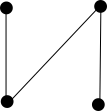
\includegraphics{imagenes/grafo_autocomplementario.png}
\end{center}

\subsubsection{}

Sabemos que $\sum_{i = 1}^{n}d(v_i) = 2m$ con $m$ la cantidad de aristas.

y que $\sum_{i = 1}^{n}d(\overline{v_i}) = \sum_{i = 1}^{n}n - 1 - d(v_i) = \sum_{i = 1}^{n}n - \sum_{i = 1}^{n}1 - \sum_{i = 1}^{n}d(v_i)$ 

Entonces $2\sum_{i = 1}^{n}d(v_i) = n^2 - n \Longleftrightarrow \sum_{i = 1}^{n}d(v_i) = \frac{n^2 - n}{2} = 2m$

Nos queda que $m = \frac{n(n - 1)}{4}$

El producto $n(n - 1)$ debe ser divisible por 4, y como no es posible que ambos sean pares, significa que uno de los factores debe ser divisible por 4. Lo que es lo mismo que $n = 4k$ ó $(n - 1) = 4k \Longleftrightarrow n = 4k + 1$

\subsection{}

\begin{codesnippet}
\begin{verbatim}
bool isomorfos?(arreglo<lista<int> U, arreglo<lista<int> V)

fin isomorfos?
\end{verbatim}
\end{codesnippet}

\subsection{}

Se copian todos los 1 en sus posiciones simetricas, es decir si $M_{ij} = M_{ji}$

\subsection{}

\subsubsection{}
$A^n$ contiene en cada elemento $A_{ij}$ la cantidad de caminos que hay de longitud $n$ desde $i$ hasta $j$.

\subsubsection{}
Sabemos que un grafo $G$ con 2 o más nodos es bipartito $\Longleftrightarrow$ no tiene circuitos simples de longitud impar.

Y también que si $A$ es la matriz de adyacencia del grafo $G$, el elemento $a^k$ de $A^k_{ij}$
es igual a la cantidad de caminos de longitud $k$ entre $i$ y $j$.

Entonces los elementos de la diagonal de $A^n$ representan la cantidad de circuitos simples de longitud $n$ para cada $A^n_{ii}$. Por lo que una diagonal nula representa que no hay circuitos simples de longitud $n$.

Por lo tanto vale que un grafo es bipartito $\Longleftrightarrow$ no tiene circuitos simples de longitud impar $\Longleftrightarrow$ la diagonal de $A^n$ con $n$ impar, es nula.

\subsection{}
Fijándose para cada $i, j$ con $1 \leq i, j \leq n$ si es posible llegar desde $i$ a $j$, si lo es se pone un 1, sino un 0. ESTO ES MALISIMO

\subsection{}
\subsubsection{}
BFS para detectar ciclos de longitud impar. La idea es que al tener el nivel de cada nodo, si se forma un ciclo y el nivel del nodo desde el que se mueve coincide en paridad con el del nodo al que llega, entonces hay un ciclo de longitud impar y no es bipartito. Si no se encuentra ninguno, es bipartito.

\begin{codesnippet}
\begin{verbatim}
bool bipartitoBFS(vector<vector<int> listaAdyacencia)

    cola<int> recorrido
    vector[n]<int> nivel
    vector[n]<bool> visitado

    // Mientras queden vertices sin visitar
    para i entre 0 y n
        si !visitado[i] entonces

            visitado[i] = verdadero
            nivel[i] = 0

            recorrido.encolar(i)
            mientras !recorrido.vacia?() hacer

                int actual = recorrido.desencolar()

                para j entre 0 y listaAdyacencia.tamaño()

                    int sucesor = listaAdyacencia[actual][j]

                    si visitado[sucesor] entonces
                        si nivel[actual] + nivel[sucesor] mod 2 == 0 entonces
                            devolver falso
                        fin si
                    sino

                        visitado[sucesor] = verdadero
                        nivel[sucesor] = nivel[actual] + 1
                        recorrido.encolar(sucesor)

                    fin si

                fin para
            fin mientras
        fin si
    fin para

    devolver verdadero

fin bipartitoBFS
\end{verbatim}
\end{codesnippet}

También se puede calcular todas las potencias impares de las matriz de adyacencia hasta $A^n$ y fijarse en la diagonal de cada una. Si se encuentra todas son nulas, es bipartito. Sino no lo es.

\subsubsection{}
Recorrer toda la matriz de adyacencia intercambiando 0s por 1s y viceversa

\subsubsection{}

\begin{itemize}
\item $\ord(n + m)$
\item $\ord(n^2)$
\end{itemize}

\subsection{}

\subsubsection{}
Cuento la cantidad de vecinos de cada vértice. Si alguno tiene un único vecino, entonces devuelvo falso. Si todos tiene 0 ó dos o mas vecinos, es verdadero.

\subsubsection{}
Primero se usa el algoritmo anterior para verificar si cada eje pertenece a un ciclo. Si es asi entonces es orientable de forma que quede fuertemente conexo, de lo contrario no lo es.

El resto del algoritmo es un DFS en el cual se da dirección a las aristas en el momento de moverse de nodo.

Elegir un nodo cualquiera.

Para ese nodo se elige un vecino y se marca su arista en direccion al mismo. Ahora se hace lo mismo para el vecino y así, recursivamente.

En algún momento se llega a un nodo ya visitado. Se vuelve en la pila de la recursión hasta encontrar un nodo al que le queden vecinos sin visitar y se vuelve a hacer el llamado recursivo para ese vecino.

\subsubsection{}
En ambos métodos lo conveniente es recibir el grafo como una lista de adyacencias.

\begin{itemize}
\item $\ord(n)$ ya que se fija en la cantidad de vecinos de cada nodo.
\item $\ord(n + m)$ ya que usa el algoritmo anterior y recorre todas las aristas, dos veces (una de ida y una de vuelta)
\end{itemize}

\subsection{}

\setcounter{subsubsection}{1}
\subsubsection{}

\begin{codesnippet}
\begin{verbatim}
maximales(vector<vector<int>> listaAdyacencia)

    vector<vector<int>> subgrafos

    mientras haya nodos sin visitar

        actual = nodoSinVisitar()
        para vecino <- actual.vecinos()

            lista<int> susVecinos = vecino.vecinos()

            // Si cada uno de sus vecinos tiene como vecino al resto y ninguno de sus vecinos 
            // marcados es vecino de actual, es un subgrafo completo maximal
            si vecinosEntreTodos?(susVecinos) && !vecinoMarcado(actual, susVecinos) entonces
                subgrafos.agregar(susVecinos + vecino + actual)
            fin si

            // Si tiene algun vecino que no sea vecino de actual, no se marca
            si todosVecinosDe(actual, susVecinos) entonces
                marcar(vecino)
            fin si

        fin para
    fin mientras

    devolver subgrafos

fin maximales
\end{verbatim}
\end{codesnippet}

\subsubsection{}
La complejidad de b. es monstruosa :)

\newpage
\section{Práctica 6}

\subsection{}

\subsubsection{}
El máximo número de vértices de un grafo conexo de 20 aristas es 21. El máximo grafo conexo que puedo formar para una cantidad fija de aristas es aquel que no tiene ciclos, es decir, un árbol.

\subsubsection{}
Sea $G$ un árbol con $m$ cantidad de ejes, siendo $m$ par. Como $G$ es árbol, tiene una cantidad de vértices $n$, talque $m = n - 1$. Por lo tanto $n$ es impar. Supongo que $G$ no tiene nodos de grado par. 

Se sabe que $2m = \sum_{i = 1}^{n}d(v_i)$. Pero la suma de los grados de los nodos no puede ser par, ya que se suman números impares una cantidad impar de veces. 

El absurdo proviene de haber supuesto que no $G$ no tiene nodos de grado par, por lo que $G$ tiene al menos un nodo de grado par y no sólo eso, sino que tiene un número impar de nodos de grado par, ya que de lo contrario la suma de los grados sería impar.

\subsection{}

\setcounter{subsubsection}{1}
\subsubsection{}

Si. Es un árbol con un eje adicional.

\subsubsection{}

Si. Un árbol con dos ejes adicionales.

\subsection{}
\subsubsection{}

Utilizaremos el siguiente teorema: 

Un grafo G con 2 o más nodos es bipartito si y sólo si no tiene circuitos simples de longitud impar.

Un árbol no trivial tiene 2 o más nodos y no tiene circuitos simples. Por lo tanto, es bipartito.

\subsubsection{}

Si, el árbol de dos vértices.

\setcounter{subsection}{4}
\subsection{}

Sabemos que $m = \frac{\sum_{i = 1}^{n}d(v_i)}{2}$ $\Longleftrightarrow$ $2m = \sum_{i = 1}^{n}d(v_i)$ y que $n \geq 2$.

Suponemos que el árbol tiene una sola hoja, osea que hay un nodo que tiene grado 1 y el resto mayor a 2.

Entonces $2m = \sum_{i = 1}^{n - 1}d(v_i) + 1$ $\Longleftrightarrow$ $2m - 1= \sum_{i = 1}^{n - 1}d(v_i)$

Sabemos también que  $d(v_i) \geq 2$ $(\forall$ $1 \leq i \leq n - 1)$

Entonces $2m - 1= \sum_{i = 1}^{n - 1}d(v_i) \geq 2(n - 1) = 2n - 2$

Como es árbol sabemos que $m = n - 1$

$2m - 1 \geq 2n - 2$

$2(n - 1) - 1 \geq 2n - 2$

$2n - 3 \geq 2n - 2$

Absurdo proveniente de suponer que el árbol tenía una sola hoja.

Para 0 hojas la demostración es igual.

\subsection{}

$\Longrightarrow$ )

$G$ es un bosque, es decir, un grafo sin ciclos. 

Una arista pertenece a un ciclo si al quitar esta arista, sus extremos pertenecen a la misma componente conexa.

Se que cualquier arista que saque de $G$ no pertenecerá a un ciclo, ya que no tiene. Entonces al sacarla sus extremos dejarán de pertenecer a la misma componente conexa formando dos componentes distintas, donde cada extremo de la arista sacada pertenece a una componente distinta.

$\Longleftarrow$ )

Al sacar cualquier eje de $G$ aumenta el número de componentes conexas. 

Entonces cualquier arista de $G$ que tome, es un puente entre dos componentes conexas distintas. Esto significa que la arista no pertenecía a un ciclo, ya que si lo hiciese, sus extremos pertenecerían a la misma componente conexa. 

Por lo tanto, $G$ no tiene ciclos.

\subsection{}
La cantidad $m$ de aristas de un árbol es $n - 1$. Por lo que la del el complemento es la cantidad total posible menos $m$. Esto es $\frac{n(n - 1)}{2} - (n - 1) = \frac{(n - 1)(n - 2)}{2}$. Esa cantidad de aristas es la misma que la de un subgrafo completo de $n - 1$ nodos. Por lo que hay dos opciones:

\begin{itemize}
\item 
El árbol contiene un nodo que tiene aristas con el resto de los nodos, su complemento deja a ese nodo sin aristas y al resto con aristas entre todos menos dicho nodo, osea un nodo asilado y un subgrafo completo.

\item
El árbol no contiene un nodo que tenga aristas con todos los demás nodos, por lo que su complemento no tiene un subgrafo completo de tamaño $n - 1$, $K_{n-1}$.
\end{itemize}

\setcounter{subsection}{8}
\subsection{}

\subsubsection{}
No porque un árbol binario tiene un número par de aristas, por ser árbol vale $m = n - 1$, por lo tanto tiene un número impar de vertices.

\subsubsection{}
$n = \sum_{i = 0}^{h}m^i$

\subsubsection{}
Un árbol $m-$ario es aquel que para el cual cada nodo tiene $m$ hijos ó es hoja. Entonces la máxima cantidad de hojas que puede tener es cuando cada nodo tiene $m$ hijos hasta llegar a tener altura $h$. Si esto se cumple cada nodo tendra $m$ hijos, $h$ veces. Por lo que la cantidad de hojas es de $m^h$.

\setcounter{subsection}{10}
\subsection{}

\subsubsection{}
Si tiene un único árbol generador, es porque no existe más de un camino para cada par de nodos, por que tampoco tiene ciclos y por lo tanto, es un árbol.

\subsubsection{}
Tomando la unión entre todos.

\subsubsection{}
Depende de la cantidad de ciclos que tenga el grafo y de sus longitudes. La cantidad de árboles generadores que pueden formarse es igual a la cantidad de combinaciones de aristas que pueden sacarse, siempre una de cada ciclo. Es necesario tener en cuenta los ciclos que comparten aristas para no repetir combinaciones.

\setcounter{subsection}{16}
\subsection{}

\subsubsection{}
Pueden contarse la cantidad de nodos recorridos a partir de un nodo cualquiera, si esa cantidad es igual a la cantidad de nodos del grafo, es conexo, sino no.

\subsection{}
Se hacen DFSs o BFSs partiendo de todos los nodos que no hayan sido marcados previamente por el algoritmo. Se cuenta esta cantidad de ``comienzos'' del algoritmo. Esa es la cantidad de componentes conexas.

\subsection{}
\subsubsection{}
Su complejidad es $\ord((n + m)$ $log$ $n)$

\setcounter{subsection}{19}
\subsection{}
Debe construirse (B,A)(A,C)(C,D)(D,E) con un largo total de 33.

\subsection{}

\subsubsection{}
Es análogo a Prim o Kruskal con la modificación de que cada nodo comienza con distancia $-\infty$ y se reemplaza por el máximo en lugar del mínimo

\subsubsection{}
El máximo árbol tiene peso total 34.

\newpage
\section{Práctica 7}

\setcounter{subsection}{1}
\subsection{}

\subsubsection{}
(A,B,1)(A,C,2)(C,B,-999)

Si Dijkstra empieza desde $A$ nunca llega a la arista (B,C) ya que hace el siguiente recorrido: (A,B)(A,C) cuando el mejor camino sería (A,C)(C,B)

\subsubsection{}
Consiste en moverse entre los nodos yendo siempre al que menor camino total represente.

\subsubsection{}
Si ya que toma la mejor decisión, osea el mínimo camino, en cada iteración.

\setcounter{subsection}{4}
\subsection{}

\subsubsection{}
Se relajan todas las aristas una última vez. Si hubo algún cambio en las distancias, entonces hay un ciclo negativo.

Si no todos los vértices son alcanzables se puede correr el algoritmo cuantas veces sea necesario para cada nodo con lognitud $\infty$. Para evitar que la complejidad del algoritmo incremente es necesario que el bucle principal finalice si es que no se detectan cambios en cuanto a la iteración anterior. De esta forma se evita repetir la relajacíon de aristas $n^2$ veces.

\newpage
\section{Práctica 8}

\setcounter{subsection}{3}
\subsection{}

$\Longrightarrow$ )

$G$ tiene un circuito euleriano, osea que si parto de un nodo $v_0$ puedo volver al mismo pasando por todas las aristas, sin repetir alguna. A su vez, todos los nodos de $G$ tienen grado par.

Puede ocurrir que $G$ sea un circuito simple, en cuyo caso tomo $G$ como la única partición, o puede que no. En ese caso puedo formar un circuito simple $C_1$ con un conjunto de aristas de $G$, ya que sé que al haber un circuito hay al menos un circuito simple.

Las aristas de $C_1$ forman un conjunto de la partición que busco. Sea $G_1 = G \setminus C_1$. Todos los vértices de $G_1$ siguen teniendo grado par. Si $G_1$ no tiene aristas ya tenemos la partición que buscábamos. Sino, seguro $G_1$ tiene un circuito simple $C_2$, por ser euleriano. Así iteramos hasta quedarnos sin aristas y nos queda la partición $\{C_1, ..., C_k\}$. \\

$\Longleftarrow$ )

$G$ puede particionarse en circuitos simples $\{C_1, ..., C_k\}$. Considero $G_0$ el grafo con los mismos nodos que $G$ pero sin aristas, sólo nodos aislados. Todos tienen grado 0, osea que todos son de grado par. Ahora agrego $C_1$. Como $C_1$ es ciclo simple, todos sus nodos tienen grado 2, por lo que agregar $C_1$ a $G_0$ forma un grafo $G_1$ en donde cada nodo aumenta de grado en 2 o permanece igual, por lo que son pares. Itero hasta agregar todos los circuitos.

El grafo que se forma es $G$, es conexo y todos sus nodos son de grado par, por lo que $G$ es un grafo euleriano.

\subsection{}

$G$ es un grafo conexo con todos sus vértices de grado par, por lo tanto es un grafo euleriano. Entonces $G$ se puede particionar en ciclos simples.

Para cualquier vértice $v \in G$ se sabe que todas sus aristas pertenecen a algún ciclo simple. Por cada arista de $v$ hay otra que también sale de $v$ que pertenece al mismo ciclo simple. Es decir que $v$ conecta $\frac{d(v)}{2}$ ciclos simples, ya que puedo elegir pares de aristas de $v$ que pertenecen al mismo ciclo.

Al sacar uno de esos pares de aristas, es posible que se forme otra componente conexa porque ese par pertenece a un ciclo simple $C$, lo que hace que se forme un camino simple ya que las aristas que elimino son adyacentes. Para formarse otra componente conexa debe ser $v$ el único nodo que une a $C$ con $G \setminus C$. Si no es así, es porque hay otro ciclo que conecta a $C$ con $G \setminus C$.

Entonces al eliminar $v$ pueden quedar a lo sumo la cantidad de ciclos simples que une $v$ de componentes conexas, es decir $\frac{d(v)}{2}$.

Por lo tanto, $w(G - v) \leq \frac{d(v)}{2}$

\setcounter{subsection}{6}
\subsection{}

\subsubsection{}

$\Longrightarrow$ )

Suponemos $G$ arbitrariamente atravesable desde $v_o$ y que $\exists C$ circuito simple que no contiene a $v_0$. Considero $G \setminus C$ (saco las aristas de $C$), donde todos los vértices tienen grado par y usando que $G$ euleriano es equivalente a $\exists$ partición de $E$ en circuitos simples, encuentro una partición en ciclos de cada componente conexa y obtengo una partición en ciclos simples de $E$ que contiene a $C$.

Recorro las aristas de todos los ciclos de la partición que contiene a $v_0$, hasta terminar en $v_0$ y no quedan ,ás aristas adyacentes a $v_0$ por recorrer. Como me falta recorrer las aristas de $C$, este circuito no es euleriano. Absurdo. \\

$\Longleftarrow$ )

Veamos que el procedimiento siempre nos da un circuito euleriano:

$G$ euleriano $\Longrightarrow$ todo vértice tiene grado par.

Al ir construyendo el circuito del procedimiento se va formando un camino en el que eventualmente se forma un ciclo $C_1$ (sino habría un vértices de grado impar) que termina en $v_0$ (sino habría un ciclo que no contiene a $v_0$).

Repitiendo el razonamiento, se forman ciclos simples disjuntos $C_1, ..., C_k$ que contienen a $v_0$ (y no hay más cuando termina el procedimiento).

Igual que antes, puedo contruir una partición de ciclos simples que contengan a $C_1$ hasta $C_k$.

Si el procedimiento no genera un circuito euleriano, $\exists$ una arista $e$ que no recorrí que pertenece a algún circuito de la partición $neq$ de los $c_i$. Absurdo porque ese circuito no contiene a $v_0$.

\subsubsection{}

Sea $C = \{C_1, ..., C_k\}$ una partición en ciclos simples de $E$. Cada ciclo aporta como mucho 2 al grado de $v$, cualquiera sea el $v \in V$ y todas las aristas están en algun ciclo $\Longrightarrow d(v) \leq 2k = d(v_0)$ ya que todo ciclo contiene a $v_0$ y son disjuntos.

\subsection{}

\subsubsection{}
Para valores impares.

\subsubsection{}
Si. $K_2$.

\subsection{}

\subsubsection{}

$\Longrightarrow$ )

Sea $G$ un digrafo conexo que tiene un circuito euleriano, es decir que tiene un circuito que recorre todas las aristas sin pasar más de una vez por cada ninguna. 

Como cada vértice $v \in G$ pertenece al circuito euleriano, por lo tanto si comienzo a recorrer el circuito partiendo desde $v$, por cada salida que tenga debe tener obligatoriamente una entrada, para poder formar el ciclo, y de la misma forma. Si no parto de $v$, por cada entrada que tenga tiene que tener una salida, para garantizar que se llegue al nodo desde donde se partió y formar el ciclo. \\

$\Longleftarrow$ )

Sea $G$ un digrafo conexo que cumple que $d_{in}(v) = d_{out}(v)$ $\forall$ vértice $v$. 

\subsection{}

Si un digrafo conexo tiene un circuito euleriano, significa que existe un ciclo dirigido que pasa por todas las aristas. Si un ciclo pasa por todas las aristas y el grafo es conexo, entonces pasa por todos los nodos. Tener un ciclo dirigido que pase por todos los nodos implica que se puede ir desde cualquier nodo a cualquier otro, siguiendo el ciclo dirigido. Lo que es lo mismo que decir que el grafo es fuertemente conexo.

\newpage
\section{Práctica 9}

\setcounter{subsection}{1}
\subsection{}



\subsection{}

\subsubsection{}
$r = m - n + c + 1$ donde $c$ es el número de componentes conexas

\subsubsection{}
Sea un grafo planar no conexo $G_N$, puedo construir un grafo planar conexo $G_C$ uniendo nodos de componentes conexas distitnas por medio de aristas. Llamemos $m_a$ a esta cantidad de aristas agregadas.

Sea $m$ la cantidad de aristas de $G_C$ y $n$ la cantidad de nodos, se cumple que $m \leq 3n - 6$. Ahora, $G_N$ tiene la misma cantidad de nodos pero $m_a$ aristas menos, es decir, $m - m_a$ aristas. Por lo tanto, $m - m_a \leq m \leq 3n - 6$.

\subsection{}

\begin{lema}
    Todo grafo planar donde todo vértice tiene grado mayor o igual a 3, se verifica que $m \leq 3r - 6$.
\end{lema}

\begin{proof}
    ~

    $3r - 6 = 3(m - n + 2) - 6 = 3m - 3n$

    Quiero ver que $m \leq 3m - 3n$

    Lo que es lo mismo que $\frac{3n}{2} \leq m$

    Como cada vértice tiene grado mayor o igual a 3, $m = \frac{\sum_{i=1}^{n}d(v_i)}{2} \geq \frac{\sum_{i=1}^{n}3}{2} = \frac{3n}{2}$.
\end{proof}

\subsection{}

\subsubsection{}
Supongo un grafo $G = (V, E)$ donde todos sus vértices tienen grado mayor o igual a 6. Como mínimo debe tener 7 nodos, todos conectados entre sí. 

Este grafo no es planar ya que no cumple con el lema \ref{planarMayor3}.

Agrego un nodo $n$ a $V$, de manera que agregue la menor cantidad de aristas posibles. Para esto voy a elegir 6 nodos $v_a, v_b, v_c, v_d, v_e, v_f \in V$ donde $(v_a, v_b), (v_c, v_d), (v_e, v_f) \in E$. Agrego al grafo las aristas $(v_a, n), (v_b, n), (v_c, n), (v_d, n), (v_e, n), (v_f, n)$ y puedo sacar $(v_a, v_b), (v_c, v_d), (v_e, v_f)$ de $E$ ya que al hacerlo cada nodo sigue vuelve a tener grado 6.

El numero de nodos aumenta en 1 y el de aristas aristas en 3. Esta es la cantidad mínima de aristas que puedo agregar por cada nodo. En principio $G$ cumplía que $m = \frac{7 \times 6}{2} = 21 = 3n$, entonces si por cada nodo que agrego la cantidad de aristas incrementa como mínimo en 3, entonces $m \geq 3n$ pero entonces $m \not \leq 3n - 6$. Lo que significa que $G$ no puede ser planar si todos sus vértices tienen grado mayor o igual a 6.

Por lo tanto un grafo planar tiene al menos un vértice de grado menor o igual a 5.

\newpage
\section{Práctica 10}

\setcounter{subsection}{1}
\subsection{}
Puede modelarse como un problema de grafos donde cada nodo es una tarea y existe una arista entre cada par de vértices que comparte un recurso.

\subsection{}
\subsubsection{}
Verdadero. Si $H$ es un subgrafo de $G \Longrightarrow \chi(H) \leq \chi(G)$. Como $\chi(K_s) = s$ y $K_s$ es subgrafo de $G$, entonces $\chi(G) \leq s$.

\subsubsection{}
Falso, por ejemplo, $C_5$.

\subsubsection{}
Falso. El subgrafo máximo completo de $C_5$ es $K_2$ mientras que su número cromático es 3. El número cromático de $K_3$ tambíen es 3.

\subsubsection{}
Falso. Puedo tener un grafo donde un vértice y sólo él se une el resto de los vértices. Su grado puede ser tan grande como quiera pero su número cromático es 2.

\subsection{}
Se agrega un nodo al grafo por cada curso en donde dos cursos comparten una arista si tienen algun inscripto en común. A partir de este modelo se colorea el grafo en donde cada color representa un horario distinto.

\subsection{}
Se arma un grafo a partir de la matriz de distancias en donde cada nodo es una torre y dos nodos comparten una arista entre sí en caso de tener una distancia mayor o igual a 50. El número cromático de este grafo es el menor número de frecuencias distintas.

\subsection{}
\setcounter{subsubsection}{1}
\subsubsection{}
Sea $G$ un grafo $k-$cromático, elijo un vértice $v in G$ tal que $G - v$ es $k-$cromático. Lo saco de $G$ e itero hasta no poder encontrar un vértice que cumpla esa condición. El grafo resultante es $k-$cromático crítico.

\subsection{}
Si $G$ es $k-$cromático y color crítico entonces:

\begin{enumerate}[label=\alph*)]
	\item {
		$G$ es conexo.

		\begin{proof}
			Supongo $G$ no conexo, $C_1, ..., C_t$ con $T \geq 2$ las componentes conexas de $G$. 

			Por lema \ref{chiMaxCC} sabemos que $\chi(G) = max \{\chi(C_i)\}_{1 \leq i \leq t}$. Entonces puedo tomar un $C_j$ tal que no sea el que tenga el número cromático máximo y sacarle un nodo, sin que disminuya el número cromático de $G$. Pero eso es absurdo porque por ser color crítico si saco un vértice su número cromático debe decrementar.
		\end{proof}
	}
	\item{
		Todo vértice de $G$ tiene grado mayor o igual a $k - 1$.

		\begin{proof}
			Supongamos que existe $v$ tal que $d(v) < k - 1$. Consideremos $G - v$. $\chi(G - v) = k - 1$ por ser color crítico.

			Entonces existe un $k-1-$coloreo $f$ de $G - v$.

			$f: V \longrightarrow \{1, ..., k - 1\}$

			Como $d(v) < k - 1$, $\exists q \in {1, ..., k - 1} / f(w) \not= q \forall w$ vecino de $v$.

			Definimos $f'$ coloreo de $G$ como $f'(v) = q$ y $f'(v) = f(w)$ sino $f'$ es $k - 1$ coloreo de $G$

			\begin{itemize}
				\item $v-w$ no traen problemas por la elección de $q$.
				\item $w-w'$ estamos(??) en $f$
			\end{itemize}

			Absurdo ($\chi(G) = k > k - 1$).
		\end{proof}
	}
	\item{
		$G$ no tiene ningún vértice que al sacarlo quede disconexo.

		\begin{proof}
			Por absurdo, supongamos que $G - v$ es no conexo.

			pendiente...
		\end{proof}
	}
\end{enumerate}

\subsection{}
\begin{prop}
	$\chi(G + H) = \chi(G) + \chi(H)$
\end{prop}

\begin{proof}
	Sean los grafos $G$ y $H$, considero $G + H$. Se que cada vértice $v_i \in G$ comparte una arista con cada vértice $u_j \in H$ debido al join. Entonces $v_i$ debe tener un color distinto a todos los $u_j$ para formar un coloreo válido. Luego, todos los $v_i$ tienen colores distintos a cualquier $u_j$, por lo que quedan $G$ y $H$ con colores distintos. Por lo tanto $\chi(G + H) = \chi(G) + \chi(H)$.
\end{proof}

\begin{cor}
	Si $G$ y $H$ son críticos, considerando $G + H$, $G$ y $H$ no comparten ningún color debido a que todos los vértices de uno comparten una arista con todos los del otro. Entonces el join no afecta al coloreo de $G$ o de $H$, se mantiene, por lo que se mantiene el color crítico de ambos. Luego, $G + H$ es color crítico.
\end{cor}

\subsection{}
\begin{lema}
	Para cualquier conjunto independiente $S$ de un grafo color critico $G$ se cumple que $\chi(G \setminus S) = \chi(G - 1)$.
\end{lema}

\begin{proof}
	Como $G$ es color crítico, cualquier vértice que saque del grafo hace que su número cromático disminuya en exactamente 1. Si tomo un conjunto independiente $S \subset G$ y elimino $S$ de $G$, es seguro que $\chi(G \setminus S) < \chi(G)$ ya que $G$ es color crítico. Ahora, como $S$ cumple la particularidad de que al ser independiente puedo asignar el mismo color a todos sus nodos puesto que no existen aristas entre dos nodos pertenecientes a $S$. Por lo tanto, se que al eliminar cualquier otro nodo que pertenezca a $S$ 
\end{proof}

\setcounter{subsection}{12}
\subsection{}
\begin{lema}
	Sea $G$ regular de $n$ nodos tal que $\chi(G) + \chi(\overline{G}) = n + 1 \Longrightarrow G = n K_1$ ó $G = K_n$ ó $G = C_n$ con $n$ impar.
\end{lema}

\begin{proof}
	
	~

	Por absurdo supongo que existe $G$ reular de $n$ nodos con $\chi(G) + \chi(\overline{G}) = n + 1$ y $G \not= n K_1$ y $G \not= K_n$ y $G$ no es $C_n$ con $n$ impar. Es decir, se cumple esto:

	\begin{enumerate}[label=\alph*)]
		\item $G$ de $n$ vértices y para algún $d$, $G$ es $d-$regular (equivalentemente $\overline{G}$ es $(n - 1 - d)-$regular).
		\item $\chi(G) + \chi(\overline{G}) = n + 1$.
		\item $G \not= n K_1$ (equivalentemente $\overline{G} \not= K_n$).
		\item $G \not= K_n$ (equivalentemente $\overline{G} \not= n K_1$).
		\item $G \not= C_n$ con $n$ impar.
	\end{enumerate}

	Quiero aplicar el teorema de Brookes a $G$ ó a $\overline{G}$. Necesito grafo conexo.

	~

	Caso 1: $G$ conexo.

	\begin{itemize}
		\item ¿$G$ es conexo? Si, por que estoy en el caso 1.
		\item ¿$G$ es no completo? Si, por d).
		\item ¿$G$ no es un ciclo impar? Si, por e).
	\end{itemize}

	$n + 1 = \chi(G) + \chi(\overline{G}) \leq \Delta(G) + \Delta(\overline{G}) + 1 = d + n - 1 - d + 1 = n$. Absurdo.

	~

	Caso 2: $G$ no conexo

	\begin{itemize}
		\item ¿$\overline{G}$ es conexo? Si, por la propiedad \ref{compConexo}.
		\item ¿$\overline{G}$ es no completo? Si, por e).
		\item {
			¿$\overline{G}$ no es un ciclo impar?

			$n = 3$ ¿$\overline{G} \not= C_3$? Si, por $G \not= 3 K_1$.

			$n \geq 5$ ¿$\overline{G} \not= C_n$ con $n$ impar? Si, por propiedad \ref{n5CicloConexo} y $G$ no conexo.
		}
	\end{itemize}
\end{proof}
\end{document}
